\documentclass[10pt,pdf,hyperref={unicode}]{beamer}

\mode<presentation>
{
\usetheme{boxes}
\beamertemplatenavigationsymbolsempty

\setbeamertemplate{footline}[page number]
\setbeamersize{text margin left=0.5em, text margin right=0.5em}
}

\usepackage[utf8]{inputenc}
\usepackage[english, russian]{babel}
\usepackage{bm}
\usepackage{multirow}
\usepackage{ragged2e}
\usepackage{indentfirst}
\usepackage{multicol}
\usepackage{subfig}
\usepackage{amsmath,amssymb}
\usepackage{enumerate}
\usepackage{mathtools}
\usepackage{comment}
\usepackage{multicol}

\usepackage[all]{xy}

\usepackage{tikz}
\usetikzlibrary{positioning,arrows}

\tikzstyle{name} = [parameters]
\definecolor{name}{rgb}{0.5,0.5,0.5}

\usepackage{caption}
\captionsetup{skip=0pt,belowskip=0pt}

\newtheorem{rustheorem}{Теорема}
\newtheorem{russtatement}{Утверждение}
\newtheorem{rusdefinition}{Определение}

% colors
\definecolor{darkgreen}{rgb}{0.0, 0.2, 0.13}
\definecolor{darkcyan}{rgb}{0.0, 0.55, 0.55}

\AtBeginEnvironment{figure}{\setcounter{subfigure}{0}}

\captionsetup[subfloat]{labelformat=empty}


%----------------------------------------------------------------------------------------------------------

\title[Исследование механизмов разрежения нейронных сетей на основе важностей весов]{Исследование механизмов разрежения нейронных сетей на основе важностей весов \\ НИР}
\author{А.\,В.\,Ребриков \\ Научный руководитель:	к.ф.-м.н., Безносиков А. Н.}

\institute[]{Московский физико-технический институт}
\date[2024]{\small 21\;декабря\;2024\,г.}

%---------------------------------------------------------------------------------------------------------
\begin{document}

\begin{frame}
\titlepage
\end{frame}

%----------------------------------------------------------------------------------------------------------


\section{Литература}
\begin{frame}{Литература}
\bibliographystyle{plain}
\bibliography{../paper/references}
\end{frame}
%----------------------------------------------------------------------------------------------------------


\section{Слайд об исследованиях}
\begin{frame}{Слайд об исследованиях}
\bigskip
Исследуется проблема регуляризации нейронных сетей засчёт рязрежения, например с помощью dropout, dropconnect.
\begin{block}{Цель исследования~---}
предложить метод разрежения нейронных сетей на основе \emph{важности} весов.
\end{block}
\begin{block}{Прелагается}
\justifying
\begin{enumerate}[1)]
\item определить \emph{важность} весов,
\item рязряжение с вероятностями, зависящими от важности весов,
\item комбинация с известными методами разрежения для получения лучших результатов.
\end{enumerate}
\end{block}
\begin{block}{Решение}
Для определения важности весов предлагается исследовать влияние изменения каждого отдельного веса в рамках одного слоя (параметра) сети на функцию ошибки.
\end{block}
\end{frame}

%---------------------------------------------------------------------------------------------------------
\section{Постановка задачи регуляризации}
\begin{frame}{Постановка задачи регуляризации}
Заданы
\begin{enumerate}[1)]
    \item признаки $a_\text{train}, a_\text{test} \in A^{n+m}$, метки $b_\text{train}, b_\text{test} \in B^{n+m} = \mathbb{R}^{r \times (n+m)}$,
    \item веса модели: $x \in X = X_1 \times X_2 \times \ldots \times X_L$,
    \item модель $f: X \times A \to B$,
    \item функция ошибки $\mathcal{L}: X \to \mathbb{R}$.
    % \item важность весов: $w \in W = W_1 \times W_2 \times \ldots \times W_L$, 
    % $\forall i \in \overline{1, L} \quad W_i = \Delta_{\dim X_i}$.
\end{enumerate}

\bigskip

При классической постановке задачи: 
\[
	\frac{1}{n} \sum_{i=1}^{n} \mathcal{L}(f(x, a_\text{train}^i), b_\text{train}^i) \to \min_{x \in X}
\]

Где решение ищется с помощью градиентного спуска.
\bigskip

Дополнительно хотим минимизировать разность с тестовой выборкой:

\[
    \text{GAP} = \frac{1}{n} \sum_{i=1}^{n} \mathcal{L}(f(x, a_\text{test}^i), b_\text{test}^i) - \frac{1}{m} \sum_{i=1}^{m} \mathcal{L}(f(x, a_\text{train}^i), b_\text{train}^i)
\]

% \bigskip
% \footnotetext[1]{\textit{Lopez-Paz D., Bottou L., Scholkopf B., Vapnik V.} Unifying distillation and privileged information // ICLR, 2016.}
% \footnotetext[2]{\textit{Hinton G., Vinyals O., Dean J.} Distilling the knowledge in a neural network // NIPS, 2015.}
\end{frame}

%----------------------------------------------------------------------------------------------------------
\section{Предложенный метод важности весов}
\begin{frame}{Предложенный метод важности весов}
~\\[-1mm]
Заданы
\begin{enumerate}[1)]
    \item признаки $a_\text{train}, a_\text{test} \in A^{n+m}$, метки $b_\text{train}, b_\text{test} \in B^{n+m} = \mathbb{R}^{r \times (n+m)}$,
    \item веса модели: $x \in X = X_1 \times X_2 \times \ldots \times X_L$,
    \item модель $f: X \times A \to B$,
    \item функция ошибки $\mathcal{L}: X \to \mathbb{R}$,
    \item важность весов: $w \in W = W_1 \times W_2 \times \ldots \times W_L$, $ W_i = |\dim X_i |\Delta_{\dim X_i}$.
\end{enumerate}

\bigskip

Поиск важности весов
\[
	\mathcal{L}(f(x -  w \odot (\gamma \nabla f), a_\text{train}^i), b_\text{train}^i) \to \min_{w \in W}
\]
где $\gamma$ -- шаг градиентного спуска.

\bigskip

Далее проводится dropconnect с вероятностями, зависящими от важности весов.

\cite{keshari2019guided}
\end{frame}

%----------------------------------------------------------------------------------------------------------
\section{Описание предложенного метода}
\begin{frame}{Описание предложенного метода}
\justifying
\begin{itemize}
\item Исследовался процесс, при котором полученные важности означали вероятность сохранения веса при dropconnect. Можно рассмотреть и другие варианты, например, наоборот, вероятность удаления веса (с надлежащим нормированием).
\item Для решения задачи поиска важности весов используется зеркальный спуск на симплексе. В качестве регуляризации используется KL-дивергенция с равномерным распределением.
\item  Эксперименты проводились на задачах классификации изображений CIFAR-10 с помощью RESNET-18.
\end{itemize}

\end{frame}


%----------------------------------------------------------------------------------------------------------
\section{Эксперименты}
\begin{frame}{Эксперименты}
\justifying

С применением регуляризации мы получаем более информативную гистограмму. Иначе зеркальный спуск сходится к вырожденному решению (выбор одного веса)

Для понимания гистограммы: в случае равномерного распределения все value равны единице, в случае вырожденного -- все value равны нулю, кроме одного.

Мы же стремимся к тому, чтобы выявить группу более важных весов.

\begin{figure}[h]
\centering
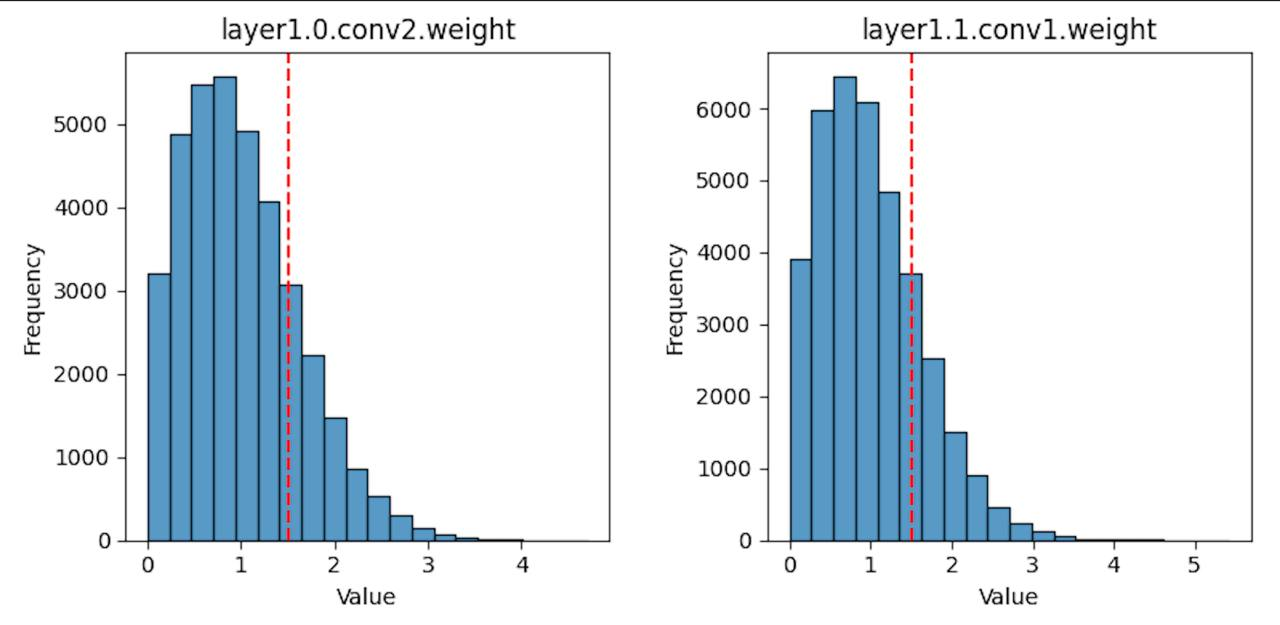
\includegraphics[width=0.8\textwidth]{../figures/impacts.jpeg}
\caption{Гистограмма важности веса (value)}
\end{figure}

\end{frame}

%----------------------------------------------------------------------------------------------------------
\section{Эксперименты}
\begin{frame}{Эксперименты}
\justifying

Сравнивались 
\begin{itemize}
\item классическое обучение модели (baseline), 
\item обучение с dropconnect на основе важности весов (impacts),
\item обучение с dropconnect на основе важности весов, но используя регуляризацию с равномерным распределением (impacts+regularization),
\item обучение с классическим dropconnect (dropconnect).
\end{itemize}
В последних трёх пунктах количество весов, которые не использовались, было одинаковым.

\begin{figure}[h]
\centering
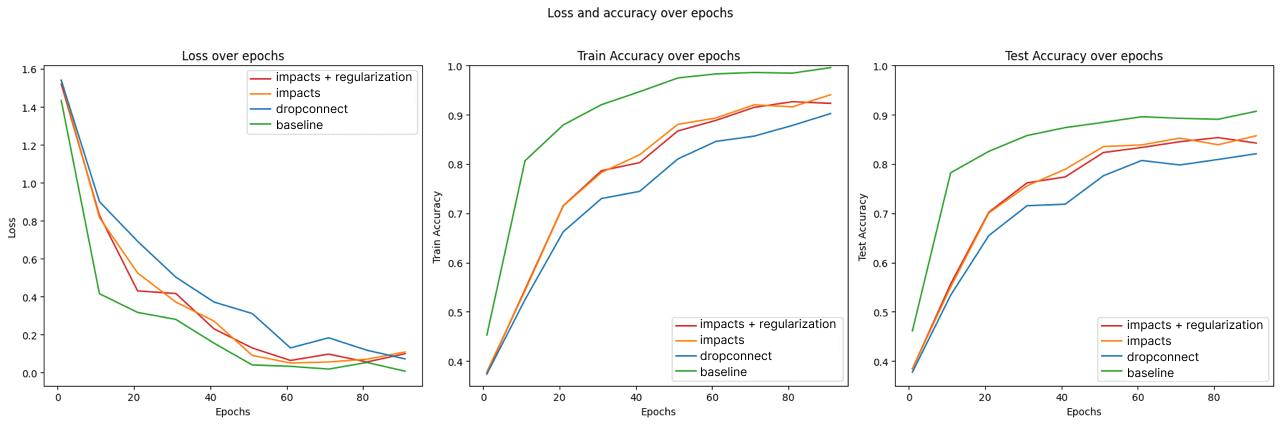
\includegraphics[width=1\textwidth]{../figures/exp.png}
\caption{Графики сходимости}
\end{figure}

\end{frame}

%----------------------------------------------------------------------------------------------------------
\section{Выводы}
\begin{frame}{Выводы}
\justifying
На текущий момент:
	\begin{enumerate}
	\justifying
        \item Предложен метод определения важности весов, основанный на зеркальном спуске на симплексе.
        \item Предложен метод регуляризации нейронных сетей: dropconnect на основе важности весов.
        \item Экспериментально показано, что предложенный метод позволяет получить лучшие результаты по сравнению с классическим dropconnect (на ранних этапах обучения).
	\end{enumerate}

\bigskip

В будущем:
\begin{enumerate}
\item Исследовать метод на поздних этапах обучения.
\item Исследовать другие подходы к разрежению на основе важности.
\end{enumerate}
\end{frame}
%----------------------------------------------------------------------------------------------------------

\end{document} 